
\documentclass[article,11pt]{article}
\usepackage{fullpage}
\usepackage{url, hyperref}
\usepackage{caption}
\usepackage{mathtools}
\usepackage{graphicx}
\usepackage{bm, amssymb}
\usepackage[explicit]{titlesec}
\usepackage{enumerate}
\usepackage{tikz}
\usepackage[makeroom]{cancel}
\newcommand{\Tt}[0]{\boldsymbol{\theta}}
\newcommand{\cc}[1]{\overline{\bf #1}}
\newcommand{\XX}[0]{{\cal X}}
\newcommand{\ZZ}[0]{{\cal Z}}
\newcommand{\va}[0]{{\vec{{\bf a}}}}
\newcommand{\vx}[0]{{\vec{{\bf x}}}}
\newcommand{\cvx}[0]{\cc{x}}
\newcommand{\vz}[0]{{\vec{{\bf z}}}}
\newcommand{\vv}[0]{{\vec{{\bf v}}}}
\newcommand{\vb}[0]{{\vec{{\bf b}}}}
\newcommand{\vq}[0]{{\vec{{\bf q}}}}
\newcommand{\vu}[0]{{\bf u}}
\newcommand{\vs}[0]{{\bf s}}
\newcommand{\vm}[0]{{\bf m}}
\newcommand{\mX}[0]{{\bf X}}
\newcommand{\mA}[0]{{\bf A}}
\newcommand{\mB}[0]{{\bf B}}
\newcommand{\mD}[0]{{\bf D}}
\newcommand{\mV}[0]{{\bf V}}
\newcommand{\mW}[0]{{\bf W}}
\newcommand{\mQ}[0]{{\bf Q}}
\newcommand{\mLbd}[0]{
    \bmx\lambda_1   & 0         & \dots & 0\\
        0           & \ddots    &       & \vdots\\
        \vdots      &           & \ddots& 0\\
        0           & \dots     & 0     & \lambda_n
    \emx
}
\newcommand{\matr}[1]{#1}
\newcommand{\vw}[0]{{\vec{{\bf w}}}}
\newcommand{\D}[0]{{\mathcal{D}}}
\newcommand{\mP}{\mathbf{P}}
\newcommand{\E}[0]{{\mathbb{E}}}
\newcommand{\vy}[0]{{\vec{{\bf y}}}}
\newcommand{\vr}[0]{{\bf r}}
\newcommand{\N}[0]{{\mathcal{N}}}
\newcommand{\vc}[0]{{\bf c}}
%\newcommand{\norm}[1]{\Vert  {#1} \Vert}
\newcommand{\norm}[1]{\left\lVert#1\right\rVert}
%\newcommand{\XX}[0]{X}
%\newcommand{\ZZ}[0]{Z}
\newcommand{\bmx}[0]{\begin{bmatrix}}
\newcommand{\emx}[0]{\end{bmatrix}}
%\newcommand{\norm}[1]{\lVert#1\rVert}
\newcommand{\T}[0]{\text{T}}
\DeclareMathOperator*{\rank}{rank}
\newcommand\defeq{:=}
\newcommand\eigvecS{\hat{\mathbf{u}}} 
\newcommand\eigvecCov{\mathbf{u}} 
\newcommand{\featuredim}{d}
\newcommand{\samplesize}{N}
\newcommand{\sampleidx}{i} 
\newcommand{\target}{y}
\newcommand{\error}{E}
\newcommand{\real}{\mathbb{R}}
\newcommand{\comp}{\mathbb{C}}
\newcommand\dataset{\mathbb{X}}
\newcommand{\inspace}{\mathcal{X}}
\newcommand{\sigmoid}{\sigma}
\newcommand{\outspace}{\mathcal{Y}}
\newcommand{\hypospace}{\mathcal{H}}
\newcommand{\emperror}{\mathcal{E}}
\newcommand{\generror}{\mathcal{E}}
\DeclareMathOperator{\supp}{supp}
%\newcommand{\loss}[3]{L({#1},{#2},{#3})} 
\newcommand{\loss}[2]{L({#1},{#2})} 
\newcommand{\determinant}[1]{{\rm det}({#1})} 
\newcommand{\prob}[1]{P({#1})}
\newcommand{\iprod}[2]{\langle#1,#2\rangle} 
\newcommand{\pdf}[1]{p({#1})}
\def \expect {\mathsf{E} }
\DeclareMathOperator*{\argmax}{argmax}
\DeclareMathOperator*{\argmin}{argmin}
\DeclareMathOperator{\spn}{span}
%\def \prob {{\rm P} }



\usepackage{amsmath,amsthm,amsfonts,mathtools}

%% Other Packages
\usepackage[most]{tcolorbox}
\usepackage[utf8]{inputenc}
\usepackage[english]{babel}
\tcbuselibrary{skins,breakable,theorems}
\usepackage[T1]{fontenc}
\usepackage{lmodern}
\usepackage{cleveref}

\tcbset{
    thmbox/.style={
        enhanced,
        breakable,
        sharp corners=all,
        fonttitle=\bfseries\normalsize,
        fontupper=\normalsize\itshape,
        leftrule=10pt,
        toprule=-1pt,
        bottomrule=-2pt,
        boxsep=5pt,
         top=0mm,
         bottom=0mm,
         right=0mm,
        colback=white,
        colframe=white,
        colbacktitle=white,
        coltitle=black,
        attach boxed title to top left,
        boxed title style={empty, size=minimal, bottom=1.5mm},
        overlay unbroken ={
            \draw (title.south west)--(title.south east);
            \draw ([xshift=3.5mm]frame.north west)|-%
                  (frame.south east)--(frame.north east);},
        overlay first={
            \draw (title.south west)--(title.south east); 
            \draw ([xshift=3.5mm]frame.north west)--([xshift=3.5mm]frame.south west);
            \draw (frame.north east)--(frame.south east);},
        overlay middle={
            \draw ([xshift=3.5mm]frame.north west)--([xshift=3.5mm]frame.south west);
            \draw (frame.north east)--(frame.south east);},
        overlay last={
            \draw ([xshift=3.5mm]frame.north west)|-%
                  (frame.south east)--(frame.north east);},
        },
    S/.style={thmbox, 
        overlay unbroken ={
            \draw (title.south west)--(title.south east);
            \draw ([xshift=3.5mm]frame.north west)--([xshift=3.5mm]frame.south west);},
        overlay first={
            \draw (title.south west)--(title.south east); 
            \draw ([xshift=3.5mm]frame.north west)--([xshift=3.5mm]frame.south west);},
        overlay middle={
            \draw ([xshift=3.5mm]frame.north west)--([xshift=3.5mm]frame.south west);},
        overlay last={
            \draw ([xshift=3.5mm]frame.north west)--([xshift=3.5mm]frame.south west);},
        },
    L/.style={thmbox, 
        overlay unbroken ={
            \draw (title.south west)--(title.south east);
            \draw ([xshift=3.5mm]frame.north west)|-([xshift=15mm]frame.south west);},
        overlay first={
            \draw (title.south west)--(title.south east); 
            \draw ([xshift=3.5mm]frame.north west)--([xshift=3.5mm]frame.south west);},
        overlay middle={
            \draw ([xshift=3.5mm]frame.north west)--([xshift=3.5mm]frame.south west);},
        overlay last={
            \draw ([xshift=3.5mm]frame.north west)|-([xshift=15mm]frame.south west);},
        },
    P/.style={thmbox,
        fonttitle=\itshape\normalsize,
        overlay unbroken ={
            \draw (title.south west)--(title.south east);
            \draw ([xshift=3.5mm]frame.north west)|-([xshift=15mm]frame.south west);
            \node[anchor=east] at (frame.south east) {$\square$};},
        overlay first={
            \draw (title.south west)--(title.south east); 
            \draw ([xshift=3.5mm]frame.north west)--([xshift=3.5mm]frame.south west);
        },
        overlay middle={
            \draw ([xshift=3.5mm]frame.north west)--([xshift=3.5mm]frame.south west);
        },
        overlay last={
            \draw ([xshift=3.5mm]frame.north west)|-([xshift=15mm]frame.south west);
            \node[anchor=east] at (frame.south east) {$\square$};
        },
    },
    M/.style={thmbox,
        fonttitle=\bfseries\Large,
        fontupper=\normalsize,
        colback=thmBgColor,
        overlay unbroken ={
            \draw (title.south west)--(title.south east);
            \draw ([xshift=3.5mm]frame.north west)--([xshift=3.5mm]frame.south west);},
        overlay first={
            \draw (title.south west)--(title.south east); 
            \draw ([xshift=3.5mm]frame.north west)--([xshift=3.5mm]frame.south west);},
        overlay middle={
            \draw ([xshift=3.5mm]frame.north west)--([xshift=3.5mm]frame.south west);},
        overlay last={
            \draw ([xshift=3.5mm]frame.north west)--([xshift=3.5mm]frame.south west);},
    },
    T/.style={thmbox,
        fonttitle=\bfseries\Large,
        fontupper=\normalsize,
        colback=thmBgColor,
        overlay unbroken ={
            \draw (title.south west)--(title.south east);
            \draw ([xshift=3.5mm]frame.north west)|-%
                (frame.south east)--(frame.north east);},
        overlay first={
            \draw (title.south west)--(title.south east); 
            \draw ([xshift=3.5mm]frame.north west)--([xshift=3.5mm]frame.south west);},
        overlay middle={
            \draw ([xshift=3.5mm]frame.north west)--([xshift=3.5mm]frame.south west);},
        overlay last={
            \draw ([xshift=3.5mm]frame.north west)--([xshift=3.5mm]frame.south west);},
    },
}

\tcbset{
    example/.style={
        enhanced,
        breakable,
        sharp corners=all,
        fonttitle=\underline\normalsize,
        fontupper=\normalsize\itshape,
         top=0mm,
         bottom=0mm,
         right=0mm,
        colback=white,
        colframe=white,
        colbacktitle=white,
        coltitle=black,
        attach boxed title to top left,
        boxed title style={empty, size=minimal, bottom=1.5mm},
        overlay unbroken ={
            \draw (title.south west)--(title.south east);
            \draw ([xshift=3.5mm]frame.north west)|-([xshift=15mm]frame.south east);},
        overlay first={
            \draw (title.south west)--(title.south east); 
            \draw ([xshift=3.5mm]frame.north west)--([xshift=3.5mm]frame.south west);
            \draw (frame.north east)--(frame.south east);},
        overlay middle={
            \draw ([xshift=3.5mm]frame.north west)--([xshift=3.5mm]frame.south west);
            \draw (frame.north east)--(frame.south east);},
        overlay last={
            \draw ([xshift=3.5mm]frame.north west)|-%
                  (frame.south east)--(frame.north east);},
        },
}

\newtcbtheorem[number within=section]{theorem}{Lause}{thmbox,T}{theo}
\newtcbtheorem[number within=section]{corollary}{Seuraus}{thmbox}{theo}
\newtcbtheorem[
    number within=section,
    crefname={definition}{Definition},
    Crefname={Definition}{Definition} ]{definition}{Definition}{thmbox,M}{theo}
\newtcbtheorem[number within=section]{lemma}{Lemma}{thmbox,M}{theo}
\newtcbtheorem[]{tcbSthmbox}{Theorem}{thmbox,S}{theo}
\newtcbtheorem[]{tcbLthmbox}{Theorem}{thmbox,L}{theo}
\newtcbtheorem[number within=section]{example}{Esimerkki}{example}{theo}

% % Theorems
\definecolor{thmBgColor}{RGB}{250,250,250}
\definecolor{thmLnColor}{RGB}{200,200,200}

% \makeatletter
% % define a new theorem style
\def\tcb@theo@widetitle#1#2#3{\hbox to \textwidth{\textsc{\large#1}\normalsize\space#3\hfil(#2)}}
\tcbset{
  theorem style/theorem wide name and number/.code={ \let\tcb@theo@title=\tcb@theo@widetitle},
  proofbox/.style={enhanced,
  breakable,
  sharp corners=all,
  fonttitle=\bfseries\normalsize,
  fontupper=\normalsize\itshape,
   top=0mm,
   bottom=0mm,
   right=0mm,
  colback=white,
  colframe=white,
  colbacktitle=white,
  coltitle=black,
  attach boxed title to top left,
  boxed title style={empty, size=minimal, bottom=1.5mm},
  overlay unbroken ={
      \draw ([xshift=3.5mm]frame.north west)|-([xshift=15mm]frame.south west);
      \node[anchor=east] at (frame.south east) {$\square$};},
  overlay first={
      \draw (title.south west)--(title.south east); 
      \draw ([xshift=3.5mm]frame.north west)--([xshift=3.5mm]frame.south west);},
  overlay middle={
      \draw ([xshift=3.5mm]frame.north west)--([xshift=3.5mm]frame.south west);},
  overlay last={
      \draw ([xshift=3.5mm]frame.north west)|-([xshift=15mm]frame.south west);
      \node[anchor=east] at (frame.south east) {$\square$};},
},
}
\newtcolorbox{ProofBox}{proofbox}
% \makeatother

% \newtcbtheorem[use counter=equation, number within=section]{mytheorem}{Theorem}%
%   {theorem style=theorem wide name and number,
%   enhanced,
%   breakable,
%   arc=0mm,
%   outer arc=0mm,
%   parbox=false,
%   boxrule=0mm,toprule=2pt,bottomrule=2pt,left=1mm,right=1mm,
%   titlerule=0mm,toptitle=0mm,bottomtitle=0mm,top=0mm,
%   colback=thmBgColor,colframe=thmLnColor,
%   title style={color=thmBgColor}, coltitle=black,
%   attach title to upper={\par\noindent},
%   before={\par\vfill\smallbreak\noindent}, after={\par},
%   fonttitle=\normalfont\large,
%   }{thm}
% \makeatother

% \newtcbtheorem[use counter=section, number within=section]{myexample}{Example}%
%   {theorem style=theorem wide name and number,
%   enhanced,
%   breakable,
%   arc=0mm,
%   outer arc=0mm,
%   parbox=false,
%   boxrule=0mm,toprule=2pt,bottomrule=2pt,left=1mm,right=1mm,
%   titlerule=0mm,toptitle=0mm,bottomtitle=0mm,top=0mm,
%   colback=thmBgColor,colframe=thmLnColor,
%   title style={color=thmBgColor}, coltitle=black,
%   attach title to upper={\par\noindent},
%   before={\par\vfill\smallbreak\noindent}, after={\par},
%   fonttitle=\normalfont\large,
%   }{thm}

% \newenvironment{example}[2][]{\noindent\myexample{#1}{#2}}{\endmyexample}

\let\realproof\proof
\let\realendproof\endproof
\renewenvironment{proof}[1][Proof]{\ProofBox\strut\textsc{#1}\space}{\endProofBox}

% %% Style Definitions
% \numberwithin{equation}{section}
\graphicspath{ {./} }
\renewcommand*{\thesection}{~\arabic{section}}
\setcounter{section}{0}
% \renewcommand*{\thesubsection}{\thesection.~\arabic{subsection}}
\renewcommand*{\thesubsubsection}{}
\renewcommand{\labelenumi}{(\alph{enumi})}

\title{CS-E4890 - Deep Learning \\ Group: FruitDealer\\ \large Project Report}
\begin{document}
\crefformat{tcb@cnt@definition}{definition~#2#1#3}
\Crefformat{tcb@cnt@Definition}{Definition~#2#1#3}

\date{}
\maketitle

\section{Problem and data description}
\begin{definition}{{\small Data }}{data}
    Project uses the dataset found in a research \href{https://www.researchgate.net/publication/321475443_Fruit_recognition_from_images_using_deep_learning}{''Fruit recognition from images using deep learning''} 
    by Horea Muresan and Mihai Oltean.
    \subsubsection{Data Properties}
    \begin{tabular}{| l | l |}
        \hline
        \bf Property & \bf value \\
        \hline			
        Total number of images & 71125 \\
    Training set size & 53177 images (one fruit per image) \\
    Test set size & 17845 images (one fruit per image) \\
    Multi-fruits set size & 103 images (more than one fruit (or fruit class) per image) \\
    Number of classes &  103 (fruits) \\
    Image size & 100x100 pixels \\
        \hline  
    \end{tabular}
    Each image is read so that each pixel's RBG value is transformed via normalization to a mean and std of 0.5.
\end{definition}
\begin{definition}{{\small Problem }}{problem}
    Goal of the project is use the data defined in \cref{theo:data} to solve a multiclass classification problem where given images are categorized to correct class by using 
    Recurrent Convolutional Neural Network.
    
    In addition to trying to solve this multiclass classification problem, project also compares this approach to Convolutional Neural Network used by Horea Muresan
    and Mihai Oltean in their research to see whether there is an improvement to be had by using a completely different Convulutional Neural Network.
\end{definition}
\begin{definition}{{\small Research Material }}{problem}
    Two research papers were used:
    \begin{enumerate}
        \item \href{https://www.researchgate.net/publication/321475443_Fruit_recognition_from_images_using_deep_learning}{"Fruit recognition from images using deep learning"} by Horea Muresan and Mihai Oltean.
        \item \href{https://www.cv-foundation.org/openaccess/content_cvpr_2015/app/2B_004.pdf}{"Recurrent Convolutional Neural Network for Object Recognition"} by Ming Liang and Xiaolin Hu.
      \end{enumerate}
\end{definition}


\newpage
\section{Method}\label{method}
As said in \cref{theo:problem} this project will focus on two methods: 
original CNN used by Horea Muresan and Mihai Oltean and RCNN described in a research 
\href{https://www.cv-foundation.org/openaccess/content_cvpr_2015/app/2B_004.pdf}{"Recurrent Convolutional Neural Network for Object Recognition"}
by Ming Liang and Xiaolin Hu.

For both cases project will use Adam Optimization Algorithm with learning rare of 0.001
and Cross Entropy Loss function for training the models.\\

\begin{definition}{{\small Convolutional Neural Network (CNN)}}{}

    Horea Muresan's and Mihai Oltean's research uses multiple different variations of dimensions in their research,
    but this project focuses on the following CNN which gave their best results:\\

    \begin{tabular}{| l | l | l |}
        \hline
        \bf Layer type & \bf Dimensions & \bf Output \\
        \hline			
        Convolutional & 5x5x4 & 16 \\
        ReLU & & \\
        Max pooling & 2 x 2 — Stride: 2 & - \\
        Convolutional & 5 x 5 x 16 & 32 \\
        ReLU & & \\
        Max pooling & 2 x 2 — Stride: 2 & - \\
        Convolutional & 5 x 5 x 32 & 64 \\
        ReLU & & \\
        Max pooling & 2 x 2 — Stride: 2 & - \\
        Convolutional & 5 x 5 x 64 & 128 \\
        ReLU & & \\
        Max pooling & 2 x 2 — Stride: 2 & - \\
        Fully connected & 5 x 5 x 128 & 1024 \\
        ReLU & & \\
        Dropout(p=0.8) & & \\
        Fully connected & 1024 & 256 \\
        ReLU & & \\
        Dropout(p=0.8) & & \\
        Softmax & 256 & 60 \\
        \hline  
    \end{tabular}\\

    So in total, 4 convulational layers, each followed by max pooling, which are then flollowed by two fully connected
    linear layers after which softmax is used to give 103 outputs (i.e. the number of classes). Linear Layers are also followed by a dropout with 0.8 probability.
\end{definition}
\begin{definition}{{\small Recurrent Convolutional Neural Network (RCNN)}}{}
    RCNN shares many similar charasteristics of normal CNN, like the name applies it uses Convolutional layers. Unlike normal CNN, all of the
    convolutional layers share the same dimensions (usually defined/indicated with variable K, i.e. RCNN-92 would indicate that it uses convolutional layers with
    dimension of 92).

    The main strucutre of RCNN is based on 5 different layers:
    \begin{tabular}{| l | l | l | l |}
        \hline
        \bf Layer & \bf Layer type & \bf Dimensions & \bf Output \\
        \hline			
        1 & Convolutional & 5 x 5 x 4 & K \\
        - & Max pooling & 3 x 3 — Stride: 2 & - \\
        2 & RCL & 3 x 3 x K — Stride: 1& -\\
        - & Dropout(p=0.8) & & - \\
        3 & RCL & 3 x 3 x K — Stride: 1 & -\\
        - & Max pooling & 3 x 3 — Stride: 2 & - \\
        - & Dropout(p=0.8) & & -\\
        4 & RCL & 3 x 3 x K — Stride: 1 & -\\
        - & Dropout(p=0.8) & & -\\
        5 & RCL & 3 x 3 x K — Stride: 1& -\\
        - & Max pooling (global) & Size of previous layer & - \\
        - & Softmax & - & 150 \\
        \hline  
    \end{tabular}\\ \\
    So each (except last) Recurrent Convolutional Layer (RCL) is followed by dropout with probability of 0.8. Max pooling is done after the first convolutional layer and at the half point of
    RCLs. Global max pooling is done after all RCLs which is then followed by softmax that gives an output with size of number of classes.

    So what is a RCL? It's a series of convulational layers with same dimensions that are repeated T times. In this project we focus on T=3 which
    means that each RCL consists total of 4 convulational layers. T=3 also provided the best results in Ming Liang's and Xiaolin Hu's research. Structure of RCL is described in the
    table below.\\
    \subsubsection{RCL}
    \begin{tabular}{| l | l | l | l |}
        \hline
        \bf T & \bf Layer type & \bf Input &\bf Notes \\
        \hline			
        0 & Convolutional & 3 x 3 x K Stride=1& No weight sharing\\
        - & ReLU & &\\
        - & BatchNorm & K-features & \\
        \hline
        \hline
        1 & Convolutional & 3 x 3 x K Stride=1 Padding=1 & weight sharing T1-T3\\
        - & ReLU & &\\
        - & T0 + T1 & & Sum of two layers\\
        - & BatchNorm & K-features &\\

        2 & Convolutional & 3 x 3 x K Stride=1 Padding=1 & weight sharing T1-T3\\
        - & ReLU & & \\
        - & T0 + T2 & & Sum of two layers\\
        - & BatchNorm & K-features & \\

        3 & Convolutional & 3 x 3 x K Stride=1 Padding=1 & weight sharing T1-T3 \\
        - & ReLU & & \\
        - & T0 + T3 & & Sum of two layers \\
        - & BatchNorm & K-features & \\
        \hline  
    \end{tabular}\\

    So T=0 differs from other of the convolutional layers a little bit. It does not share the weights with the other layers, while
    T=1-3 use the same weights for each layer. In addition, in T=1-3 we also add T=0 layer to our current layer before we move to next one.
    
    For this project, K=32 is chosen since video card memory would not be enough to support much bigger dimensions.
\end{definition}

Project could have chosen different parameters for these models and test out different variations, but unfortunately
it did not fit to the scope of this project. Because of this, project focuses on the best models found in each research material and uses
parameters that can be supported with 12GB of Video RAM.

\section{Experiments and results}
Since we want to get as comparable results as possible, project built both models described in section~\ref{method} (which can be looked into in section~\ref{code}).
In both cases project used Adam Optimization Algorithm with learning rate of 0.001 and Cross Entropy Loss for training the models.

For CNN, training configured to batch size of 60 which was run 75 epochs. As for RCNN,
batch size of 150 was chosen and it was run only 10 epochs.
Training and Validation sets were done using the original data split
defined in \cref{theo:data}.

This training setup resulted following accuracy curves visualized in a plot:

\begin{center}
    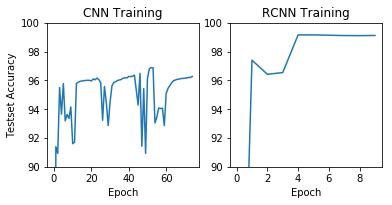
\includegraphics[width=0.5\textwidth]{training}
    \captionof{figure}{Training results of CNN and RCNN}
    \label{fig:training}
\end{center}

From which we can extract best and final results for each training and compare it to the research:\\

\tiny{\begin{tabular}{| l | c | c | c | c | c |}
    \hline
    & \bf \begin{tabular}{@{}c@{}}H. Muresan's and \\ M. Oltean's Research\end{tabular}
        & \bf \begin{tabular}{@{}c@{}}CNN Pytorch \\(best)\end{tabular}
        & \bf \begin{tabular}{@{}c@{}}CNN Pytorch \\(final)\end{tabular}
        & \bf \begin{tabular}{@{}c@{}}RCNN Pytorch \\(best)\end{tabular}
        & \bf \begin{tabular}{@{}c@{}}RCNN Pytorch \\(final)\end{tabular}\\
    \hline
    \bf\begin{tabular}{@{}c@{}}Validation Set\\Accuracy\end{tabular} & 95.88\% & 96.90\% & 96.27\% & 99.16\%& 99.12\% \\
    \hline
\end{tabular}}\\
\\ \normalsize
From these results we can see quite significant improvement in test set where we can see over 2\% improvement
over the Pytorch reimplementation of H. Muresan’s and M. Oltean’s Research and the research itself. Pytorch implementation seems
to do slightly better than indicated in the research paper, but arguably not significant.

However, while CNN was able to take full power of the GPU, current RCNN Pytorch implementation was able to take advantage about 17\% of the Nvidia 2080 TI, leading to believe
that some preprocessing steps could bring huge improvements to the training performance of the model. However due to the scope of this project these
improvements were left out. For RCNN, easy fixes to batch size and RCNN dimension sizes only affected how much of memory the model will eat up.
Though, even this observation would require much more thorough investigation which is out of scope for this project.

\section{Conclusions}

RCNN-32 was able to outperform tradition CNN with quite significant margin, with quite small layer dimensionality, so there might be further 
improvements to be had by using even bigger dimensions or tweaking other parameters of the network.

Coding the RCNN model also proved to be little more challenging than I expected. Even though the dimensions of the network are quite
simple, the Pytorch implementation of RCL is not as clear cut as it would be with either Tensorflow or Keras.
This is especially true when you have to use weight sharing for RCL's layers or figuring out padding and strides for some of the layers (where as in Tensorflow or Keras you could use keyword "same").
But as it is with deeper (i.e. more layers in total) networks, it's more challenging to check that each part is implemented correctly.

Code could also be improved by saving the best x models during the execution and picking up the the best one (i.e. best validation/test accuracy) after all iterations have finished. Now it only saves
the last one.

\section{Code}\label{code}
Code for RCNN and CNN implementation are added to the end of this report. For easier reading, you can also look them up in Github.\\

\begin{tabular}{| l | l |}
    \hline
    \bf Description & \bf URL \\
    \hline
    \begin{tabular}{@{}c@{}}Repository containing all the files \\and environment used for this project\end{tabular}
     & \href{https://github.com/Sefriol/deeplearning_project}{Repository} \\
    \hline
    pretrained RCNN Model & \href{https://github.com/Sefriol/deeplearning_project/blob/master/project/rcnn.pth}{RCNN Model} \\
    \hline
    pretrained RCNN Model & \href{https://github.com/Sefriol/deeplearning_project/blob/master/project/cnn.pth}{CNN Model} \\
    \hline
    RCNN Code & \href{https://github.com/Sefriol/deeplearning_project/blob/master/project/RCNN.ipynb}{RCNN Model} \\
    \hline
    CNN Code & \href{https://github.com/Sefriol/deeplearning_project/blob/master/project/CNN.ipynb}{CNN Model} \\
    \hline
\end{tabular}

\end{document}